For the simplicity of reading, we will take some new notation convention during this chapter:\\
\begin{itemize}
 \item Matrix: Uppercase  \textbf{A}
 \item Vector: Lower-case  \textbf{a}
 \item Scalar: Lower-case a
 \item 2D convolution operation : *
 \item $D \times D$ identity matrix: \textbf{$I_D$}
 \item Kronecker product : $\odot$
 \item $D \times D$ Fourier matrix : \textbf{F}
 \item Hadamard product: $\otimes$
 \item inverse FFT : $ \mathcal{F}^{-1}$
 \item Mapping function that preserve only $M \ll D$ active values relating to the small spatial structure of the estimated filter : $ \mathcal{M}\{\}$
\end{itemize} 


\section{Idea}
\begin{figure}[h]
 \centering
 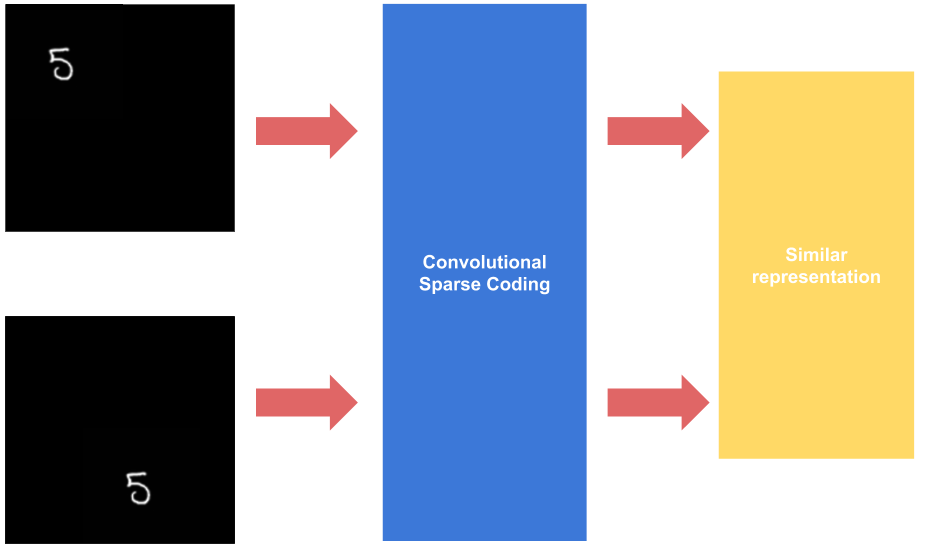
\includegraphics[scale=0.3]{csc_idea.png}
 % csc_idea.png: 926x551 px, 72dpi, 32.67x19.44 cm, bb=0 0 926 551
 \caption{Idea behind Convolutional Sparse Coding}
 \label{fig:csc_idea}
\end{figure}
In signal processing, shift variance is an important factor to consider. Indeed, there are no guarantees that the searched pattern is at the same location in the signal.\\
Based on Sparse Coding, other algorithms like Efficient Shift-Invariant Dictionary learning \cite{Zheng:2016:ESD:2939672.2939824} or Convolutional Sparse Coding \cite{6618901} refers to the problem of finding a set of latent basis vectors that capture informative \textit{local patterns} at different locations in the input sequence and not in the entire input sequence (example in figure \ref{fig:csc_idea}).\\
Among these two methods, we choose to use Convolutional Sparse coding because of the Shift-invariant power of convolution.

\subsection{Problem formulation}
\begin{figure}[h]
 \centering
 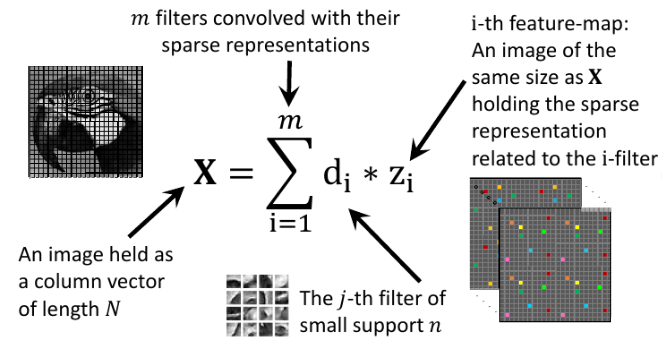
\includegraphics[scale=0.7]{CSC_superslide.png}
 % CSC_superslide.png: 662x351 px, 96dpi, 17.51x9.29 cm, bb=0 0 496 263
 \caption{CSC principle by Michael Elad \protect\footnotemark}
 \label{fig:CSC_slide}
\end{figure}
\footnotetext{\url{https://elad.cs.technion.ac.il/wp-content/uploads/2018/07/ICML_Talk_July_2018.pdf}}

Instead  of decomposing a signal as $x = D\gamma$, Convolutional Sparse Coding is the summation of convolutions between feature map $z$ (i.e. which refer to $\gamma$ in the traditional sparse coding) and the corresponding filter $d$ (i.e. our atoms in the dictionary in traditional Sparse Coding) in the dictionary $D$ (figures \ref{fig:CSC_slide} and \ref{fig:CSC_test}). So we have:\\
\begin{center}
 $X = \sum_{i=1}^{m} d_i * Z_i$\\  \vspace{0.4cm}
  $\underset{d, z}{\argmin}  \frac{1}{2} \| x - \sum_{k=1}^{K} d_k * z_k \|_2^2 + \beta \|z_k \|_1$\\

\end{center}
\begin{figure}[h]
 \centering
 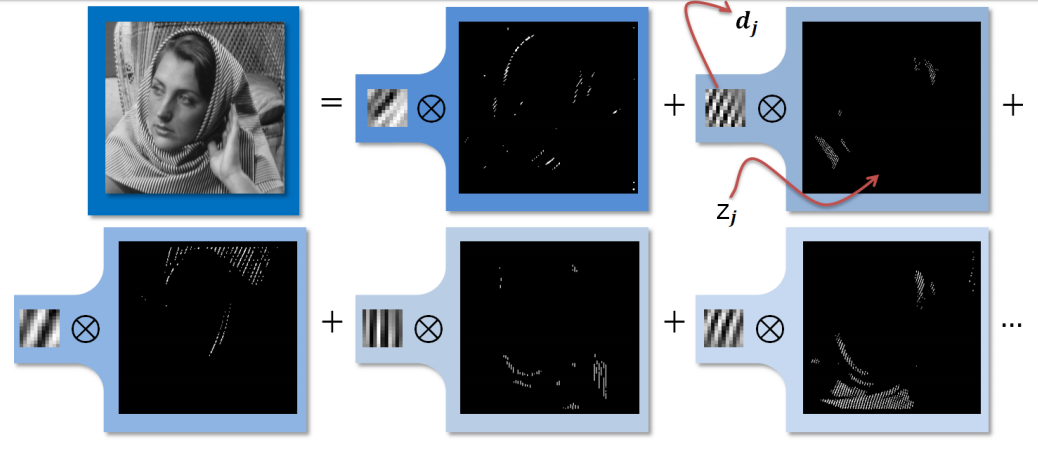
\includegraphics[scale=1.5]{CSC_test.png}
 % CSC_test.png: 1038x468 px, 300dpi, 8.79x3.96 cm, bb=0 0 249 112
 \caption{Example of reconstruction using atoms $d_j$ and features map $z_j$\protect\footnotemark}
 \label{fig:CSC_test}
\end{figure}
\footnotetext{\url{http://jsulam.cswp.cs.technion.ac.il/wp-content/uploads/sites/27/2017/12/Presentation_Handout.pdf}}
This new approach assumes that all input vectors X are independent of each other. But the complexity of convergence dramatically increases.
Bristow \cite{6618901} proposed an Augmented Lagrangian and the use of  Alternative Direction Method of Multipliers (ADMM) to solve this problem. His approach is based on three key points:
\begin{itemize}
 \item The use of ADMM
 \item The convolution subproblem can be solved efficiently (and explicitly) in the Fourier domain (instead of temporal domain)
\item The use of quad-decomposition of the objective into four subproblems (which are convex)
\end{itemize}
In this approach, to solved a Convolutional Sparse Coding problem they introduced two auxiliary variables: \textbf{t} and \textbf{s} and posing the objective in the Fourier domain:
\begin{center}
$\underset{d, s, z, t}{\argmin} \hspace{0.4cm} \frac{1}{2D} \| \hat{x} - \sum_{k=1}^{K} \hat{d}_{k} \odot \hat{z}_k \|^2_2 + \beta \sum_{k=1}^{K} \|t_k\|_1$\\
subject to $\hspace{0.4cm} \|s_k\|^2_2 \leq 1 $ for k = 1.. K\\
                $ \hspace{2.4cm}s_k = \Phi^T \hat{d}_k$ for k = 1..K\\
                $\hspace{1.9cm}z_k = t_k$ for k = 1..K
\end{center}
With $\Phi$ a D $\times$ M submatrix of the Fourier matrix $F = [\Phi,\Phi_\bot]$. In this formulation $\hat{d}_k$ is a D-dimensional vector whereas in the original formulation $d_k \in \R^M$  is of a significantly smaller dimensionality to $M \ll D$  corresponding to its smaller spatial support. 
